\section{Introducción}
\begin{frame}{Introducción - Punto de vista newtoniano}
\begin{minipage}{0.45\linewidth}
    La mecánica newtoniana es un modelo físico
que funciona para describir la dinámica de los cuerpos en el espacio por medio
de las fuerzas que contiene cada objeto. Históricamente, la mecánica newtoniana
fue el primer modelo físico en poder representar de buena manera la dinámica de
los objetos al punto de predecir acciones importantes sobre el movimiento de los
cuerpos, en donde se incluyen las trayectorias de ciertos planetas.
\end{minipage}
\hspace{1cm}
\begin{minipage}{0.45\linewidth}
    \begin{equation*}
        \dot{p}=\frac{d(mv)}{dt} = F, \qquad \left\lbrace\begin{matrix}
            \dot{p}_x= \frac{d(m_x)}{dt} = F_x \\ \\
            \dot{p}_y= \frac{d(m_y)}{dt} = F_y \\ \\
            \dot{p}_z= \frac{d(m_z)}{dt} = F_z   \\ \\
        \end{matrix} \right.
    \end{equation*}
\end{minipage}
\end{frame}
\begin{frame}{Introducción - Sistemas de cuerpos}
    El problema físico clásico puede plantearse de forma simplificada como:\vspace{1cm}\\
    \textit{Dadas las propiedades orbitales (masa, posición instantánea y velocidad) de un grupo
    de cuerpos astronómicos, determinar las fuerzas interactivas actuantes; y consiguientemente, calcular sus movimientos orbitales para cualquier instante futuro.}
\end{frame}
\begin{frame}{Introducción - Sistemas binarios}
    \begin{minipage}{0.70\linewidth}
        En astronomía, el término sistema binario se utiliza para referirse a dos objetos 
        astronómicos que orbitan alrededor de un centro de masa común debido a la fuerza
        gravitatoria que hay dada su cercanía. Normalmente se utiliza para referirse a dos
        estrellas, sin embargo, el término puede aplicarse a un sistema formado por un
        planeta y un satélite natural, siempre y cuando este último sea excepcionalmente
        grande en comparación con el planeta. Algunos ejemplos de estos son:
        \begin{itemize}
            \item La galaxia de Bode (M81) y la galaxia del Cigarro (M82).
            \item Dentro del sistema solar, el sistema Plutón-Caronte está formado por un
            planeta y un satélite.
        \end{itemize}
    \end{minipage}
    \hspace{1cm}
    \begin{minipage}{0.20\linewidth}
        \vspace{0.5cm}
        \begin{figure}[H]
            \centering
            \begin{subfigure}{1\linewidth}
                \centering
                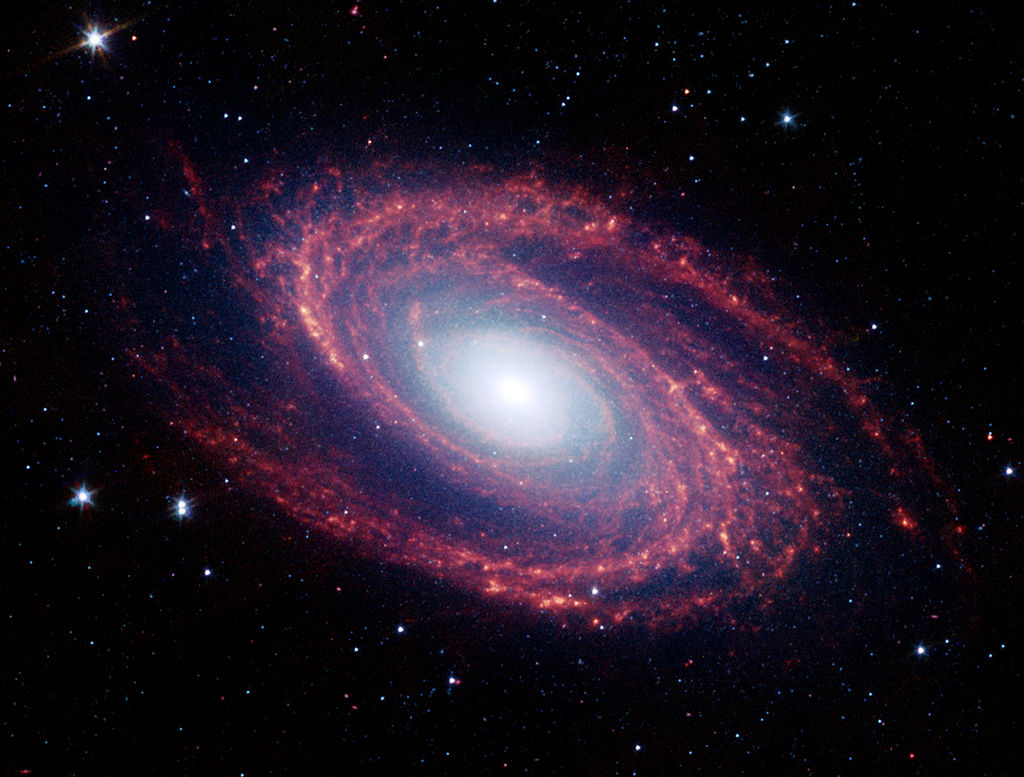
\includegraphics[scale=0.3]{images/bode.jpg}
                \caption{Galaxia de Bode}
            \end{subfigure}
            \begin{subfigure}{1\linewidth}
                \centering
                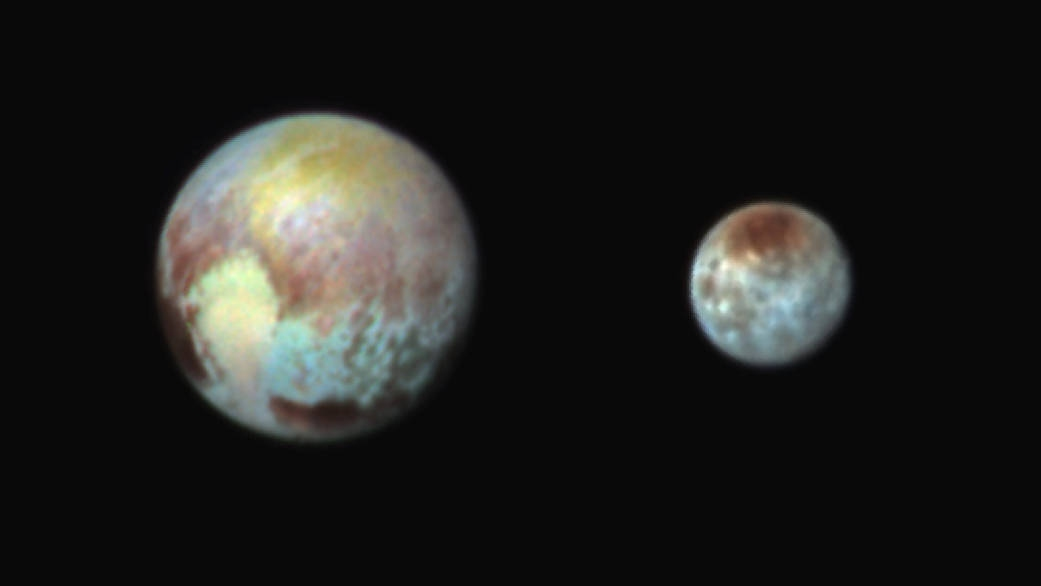
\includegraphics[scale=0.07]{images/caronte.jpg}
                \caption{Pluton y caronte}
            \end{subfigure}
            \caption{Ejemplos de sistemas binarios}
        \end{figure}
    \end{minipage}
    \end{frame}
\begin{frame}{Introducción - Origen y principios de la relatividad general}
    Las características esenciales de la teoría de la relatividad general son las siguien-
tes:
\begin{itemize}
\item El principio general de covariancia: las leyes de la Física deben tomar la
misma forma matemática en todos los sistemas de coordenadas.
\item El principio de equivalencia o de invariancia local de Lorentz: las leyes de
la relatividad especial (espacio plano de Minkowski) se aplican localmente
para todos los observadores inerciales.
\item La curvatura del espacio-tiempo es lo que observamos como un campo gravitatorio,
 en presencia de materia la geometría del espacio-tiempo no es plana
  sino curva, una partícula en movimiento libre inercial en el seno de un
campo gravitatorio sigue una trayectoria geodésica.
\end{itemize}
\end{frame}